% Generated by Sphinx.
\def\sphinxdocclass{report}
\documentclass[letterpaper,10pt,english]{sphinxmanual}

        \usepackage{ucs}
        \usepackage[utf8x]{inputenc}

\usepackage[T1]{fontenc}
\usepackage{babel}
\usepackage{times}
\usepackage[Bjarne]{fncychap}
\usepackage{longtable}
\usepackage{sphinx}
\usepackage{multirow}

    \usepackage{wrapfig}
    \usepackage{caption}
    \captionsetup{justification=raggedleft,singlelinecheck=false}

\title{Create Slideshows and Galleries Documentation}
\date{January 13, 2012}
\release{7.x-1.x-dev}
\author{Melissa Anderson \textless{}eliza411\textgreater{}}
\newcommand{\sphinxlogo}{
\includegraphics{opensourcery.png}\par}
\renewcommand{\releasename}{Release}
\makeindex

\makeatletter
\def\PYG@reset{\let\PYG@it=\relax \let\PYG@bf=\relax%
    \let\PYG@ul=\relax \let\PYG@tc=\relax%
    \let\PYG@bc=\relax \let\PYG@ff=\relax}
\def\PYG@tok#1{\csname PYG@tok@#1\endcsname}
\def\PYG@toks#1+{\ifx\relax#1\empty\else%
    \PYG@tok{#1}\expandafter\PYG@toks\fi}
\def\PYG@do#1{\PYG@bc{\PYG@tc{\PYG@ul{%
    \PYG@it{\PYG@bf{\PYG@ff{#1}}}}}}}
\def\PYG#1#2{\PYG@reset\PYG@toks#1+\relax+\PYG@do{#2}}

\def\PYG@tok@gd{\def\PYG@tc##1{\textcolor[rgb]{0.63,0.00,0.00}{##1}}}
\def\PYG@tok@gu{\let\PYG@bf=\textbf\def\PYG@tc##1{\textcolor[rgb]{0.50,0.00,0.50}{##1}}}
\def\PYG@tok@gt{\def\PYG@tc##1{\textcolor[rgb]{0.00,0.25,0.82}{##1}}}
\def\PYG@tok@gs{\let\PYG@bf=\textbf}
\def\PYG@tok@gr{\def\PYG@tc##1{\textcolor[rgb]{1.00,0.00,0.00}{##1}}}
\def\PYG@tok@cm{\let\PYG@it=\textit\def\PYG@tc##1{\textcolor[rgb]{0.25,0.50,0.56}{##1}}}
\def\PYG@tok@vg{\def\PYG@tc##1{\textcolor[rgb]{0.73,0.38,0.84}{##1}}}
\def\PYG@tok@m{\def\PYG@tc##1{\textcolor[rgb]{0.13,0.50,0.31}{##1}}}
\def\PYG@tok@mh{\def\PYG@tc##1{\textcolor[rgb]{0.13,0.50,0.31}{##1}}}
\def\PYG@tok@cs{\def\PYG@tc##1{\textcolor[rgb]{0.25,0.50,0.56}{##1}}\def\PYG@bc##1{\colorbox[rgb]{1.00,0.94,0.94}{##1}}}
\def\PYG@tok@ge{\let\PYG@it=\textit}
\def\PYG@tok@vc{\def\PYG@tc##1{\textcolor[rgb]{0.73,0.38,0.84}{##1}}}
\def\PYG@tok@il{\def\PYG@tc##1{\textcolor[rgb]{0.13,0.50,0.31}{##1}}}
\def\PYG@tok@go{\def\PYG@tc##1{\textcolor[rgb]{0.19,0.19,0.19}{##1}}}
\def\PYG@tok@cp{\def\PYG@tc##1{\textcolor[rgb]{0.00,0.44,0.13}{##1}}}
\def\PYG@tok@gi{\def\PYG@tc##1{\textcolor[rgb]{0.00,0.63,0.00}{##1}}}
\def\PYG@tok@gh{\let\PYG@bf=\textbf\def\PYG@tc##1{\textcolor[rgb]{0.00,0.00,0.50}{##1}}}
\def\PYG@tok@ni{\let\PYG@bf=\textbf\def\PYG@tc##1{\textcolor[rgb]{0.84,0.33,0.22}{##1}}}
\def\PYG@tok@nl{\let\PYG@bf=\textbf\def\PYG@tc##1{\textcolor[rgb]{0.00,0.13,0.44}{##1}}}
\def\PYG@tok@nn{\let\PYG@bf=\textbf\def\PYG@tc##1{\textcolor[rgb]{0.05,0.52,0.71}{##1}}}
\def\PYG@tok@no{\def\PYG@tc##1{\textcolor[rgb]{0.38,0.68,0.84}{##1}}}
\def\PYG@tok@na{\def\PYG@tc##1{\textcolor[rgb]{0.25,0.44,0.63}{##1}}}
\def\PYG@tok@nb{\def\PYG@tc##1{\textcolor[rgb]{0.00,0.44,0.13}{##1}}}
\def\PYG@tok@nc{\let\PYG@bf=\textbf\def\PYG@tc##1{\textcolor[rgb]{0.05,0.52,0.71}{##1}}}
\def\PYG@tok@nd{\let\PYG@bf=\textbf\def\PYG@tc##1{\textcolor[rgb]{0.33,0.33,0.33}{##1}}}
\def\PYG@tok@ne{\def\PYG@tc##1{\textcolor[rgb]{0.00,0.44,0.13}{##1}}}
\def\PYG@tok@nf{\def\PYG@tc##1{\textcolor[rgb]{0.02,0.16,0.49}{##1}}}
\def\PYG@tok@si{\let\PYG@it=\textit\def\PYG@tc##1{\textcolor[rgb]{0.44,0.63,0.82}{##1}}}
\def\PYG@tok@s2{\def\PYG@tc##1{\textcolor[rgb]{0.25,0.44,0.63}{##1}}}
\def\PYG@tok@vi{\def\PYG@tc##1{\textcolor[rgb]{0.73,0.38,0.84}{##1}}}
\def\PYG@tok@nt{\let\PYG@bf=\textbf\def\PYG@tc##1{\textcolor[rgb]{0.02,0.16,0.45}{##1}}}
\def\PYG@tok@nv{\def\PYG@tc##1{\textcolor[rgb]{0.73,0.38,0.84}{##1}}}
\def\PYG@tok@s1{\def\PYG@tc##1{\textcolor[rgb]{0.25,0.44,0.63}{##1}}}
\def\PYG@tok@gp{\let\PYG@bf=\textbf\def\PYG@tc##1{\textcolor[rgb]{0.78,0.36,0.04}{##1}}}
\def\PYG@tok@sh{\def\PYG@tc##1{\textcolor[rgb]{0.25,0.44,0.63}{##1}}}
\def\PYG@tok@ow{\let\PYG@bf=\textbf\def\PYG@tc##1{\textcolor[rgb]{0.00,0.44,0.13}{##1}}}
\def\PYG@tok@sx{\def\PYG@tc##1{\textcolor[rgb]{0.78,0.36,0.04}{##1}}}
\def\PYG@tok@bp{\def\PYG@tc##1{\textcolor[rgb]{0.00,0.44,0.13}{##1}}}
\def\PYG@tok@c1{\let\PYG@it=\textit\def\PYG@tc##1{\textcolor[rgb]{0.25,0.50,0.56}{##1}}}
\def\PYG@tok@kc{\let\PYG@bf=\textbf\def\PYG@tc##1{\textcolor[rgb]{0.00,0.44,0.13}{##1}}}
\def\PYG@tok@c{\let\PYG@it=\textit\def\PYG@tc##1{\textcolor[rgb]{0.25,0.50,0.56}{##1}}}
\def\PYG@tok@mf{\def\PYG@tc##1{\textcolor[rgb]{0.13,0.50,0.31}{##1}}}
\def\PYG@tok@err{\def\PYG@bc##1{\fcolorbox[rgb]{1.00,0.00,0.00}{1,1,1}{##1}}}
\def\PYG@tok@kd{\let\PYG@bf=\textbf\def\PYG@tc##1{\textcolor[rgb]{0.00,0.44,0.13}{##1}}}
\def\PYG@tok@ss{\def\PYG@tc##1{\textcolor[rgb]{0.32,0.47,0.09}{##1}}}
\def\PYG@tok@sr{\def\PYG@tc##1{\textcolor[rgb]{0.14,0.33,0.53}{##1}}}
\def\PYG@tok@mo{\def\PYG@tc##1{\textcolor[rgb]{0.13,0.50,0.31}{##1}}}
\def\PYG@tok@mi{\def\PYG@tc##1{\textcolor[rgb]{0.13,0.50,0.31}{##1}}}
\def\PYG@tok@kn{\let\PYG@bf=\textbf\def\PYG@tc##1{\textcolor[rgb]{0.00,0.44,0.13}{##1}}}
\def\PYG@tok@o{\def\PYG@tc##1{\textcolor[rgb]{0.40,0.40,0.40}{##1}}}
\def\PYG@tok@kr{\let\PYG@bf=\textbf\def\PYG@tc##1{\textcolor[rgb]{0.00,0.44,0.13}{##1}}}
\def\PYG@tok@s{\def\PYG@tc##1{\textcolor[rgb]{0.25,0.44,0.63}{##1}}}
\def\PYG@tok@kp{\def\PYG@tc##1{\textcolor[rgb]{0.00,0.44,0.13}{##1}}}
\def\PYG@tok@w{\def\PYG@tc##1{\textcolor[rgb]{0.73,0.73,0.73}{##1}}}
\def\PYG@tok@kt{\def\PYG@tc##1{\textcolor[rgb]{0.56,0.13,0.00}{##1}}}
\def\PYG@tok@sc{\def\PYG@tc##1{\textcolor[rgb]{0.25,0.44,0.63}{##1}}}
\def\PYG@tok@sb{\def\PYG@tc##1{\textcolor[rgb]{0.25,0.44,0.63}{##1}}}
\def\PYG@tok@k{\let\PYG@bf=\textbf\def\PYG@tc##1{\textcolor[rgb]{0.00,0.44,0.13}{##1}}}
\def\PYG@tok@se{\let\PYG@bf=\textbf\def\PYG@tc##1{\textcolor[rgb]{0.25,0.44,0.63}{##1}}}
\def\PYG@tok@sd{\let\PYG@it=\textit\def\PYG@tc##1{\textcolor[rgb]{0.25,0.44,0.63}{##1}}}

\def\PYGZbs{\char`\\}
\def\PYGZus{\char`\_}
\def\PYGZob{\char`\{}
\def\PYGZcb{\char`\}}
\def\PYGZca{\char`\^}
\def\PYGZsh{\char`\#}
\def\PYGZpc{\char`\%}
\def\PYGZdl{\char`\$}
\def\PYGZti{\char`\~}
% for compatibility with earlier versions
\def\PYGZat{@}
\def\PYGZlb{[}
\def\PYGZrb{]}
\makeatother

\begin{document}

\maketitle
\tableofcontents
\phantomsection\label{index::doc}


Contents:

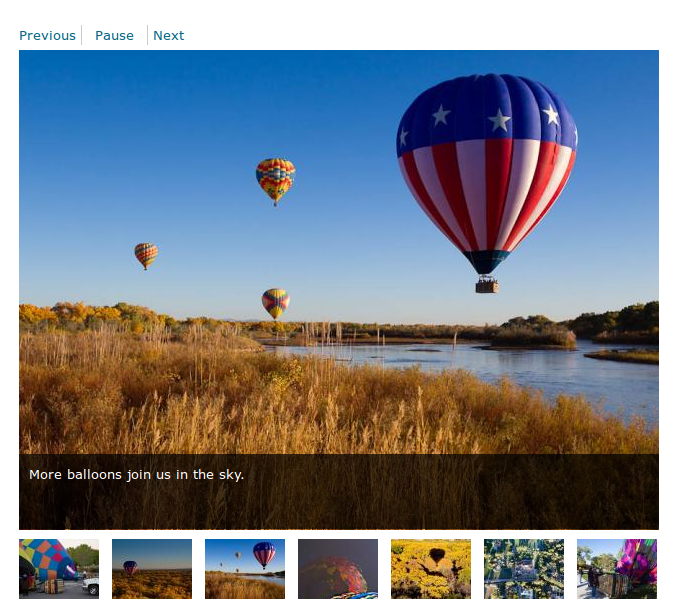
\includegraphics{balloons.png}


\chapter{Ingredients}
\label{slideshows::doc}\label{slideshows:welcome-to-create-slideshows-and-galleries-s-documentation}\label{slideshows:ingredients}

\section{Staple}
\label{slideshows:staple}\begin{enumerate}
\item {} 
\href{http://drupal.org/project/ctools}{http://drupal.org/project/ctools} - Enable Chaos Tools (all others are not needed)

\item {} 
\href{http://drupal.org/project/views}{http://drupal.org/project/views} - Enable Views and Views UI

\item {} 
\href{http://drupal.org/project/libraries}{http://drupal.org/project/libraries} - Enable Libraries

\item {} 
\href{http://drupal.org/project/views\_slideshow}{http://drupal.org/project/views\_slideshow} - Enable Views Slideshow

\end{enumerate}


\section{Theme}
\label{slideshows:theme}
Because this recipe requires custom theming, we're using Adaptive Themes (which makes the site mobile-friendly), Corolla (which makes it attractive), and Footheme (which provide a ready-to-customize subtheme). This choice facilitates best practices in custom theming and isn't required for any of the actual functionality.
\begin{enumerate}
\item {} 
\href{http://drupal.org/project/adaptivetheme}{http://drupal.org/project/adaptivetheme}

\item {} 
\href{http://drupal.org/project/corolla}{http://drupal.org/project/corolla}

\item {} 
\href{http://drupal.org/project/footheme}{http://drupal.org/project/footheme}

\end{enumerate}

At Appearance, set footheme as the default.

\textbf{Drush users:}

\begin{Verbatim}[commandchars=\\\{\}]
drush dl ctools views libraries views\_slideshow adaptivetheme corolla footheme
drush en ctools views views\_ui libraries views\_slideshow views\_slideshow\_cycle -y
\end{Verbatim}


\section{Speciality}
\label{slideshows:speciality}
The Views Slideshow module uses two external libraries.
\begin{quote}

Required for basic slideshow functionality:
\begin{enumerate}
\item {} 
Visit \href{http://malsup.com/jquery/cycle/download.html}{http://malsup.com/jquery/cycle/download.html}

\item {} 
Click the link to “Cycle Plugin”

\item {} 
In your browser, choose File \textgreater{} Save Page as \textgreater{} jquery.cycle.all.js

\item {} 
Place in sites/all/libraries/jquery.cycle (you'll have to create that folder) so that the final path looks like sites/all/libraries/jquery.cycle/jquery.cycle.all.js

\end{enumerate}

Required for advanced features, which include setting the speed of the slideshow:
\begin{enumerate}
\item {} 
Visit \href{https://github.com/douglascrockford/JSON-js/downloads}{https://github.com/douglascrockford/JSON-js/downloads} and download the appropriate format, .zip or .tar.gz, for your environment.

\item {} 
Extract it

\item {} 
Rename the directory (which begins with douglascrockford-) to json2

\item {} 
Place it in sites/all/libraries so that the final path looks like: sites/all/libraries/json2/json2.js

\end{enumerate}
\end{quote}


\chapter{Build the form for creating galleries}
\label{slideshows:build-the-form-for-creating-galleries}

\section{Add a new content type called Gallery}
\label{slideshows:add-a-new-content-type-called-gallery}
\emph{Structure \textgreater{} Content types \textgreater{} +Add new content type}
\begin{enumerate}
\item {} 
Name: Gallery

\item {} 
Description: Create an image gallery with slideshow controls.

\item {} 
Set the following values:

\begin{tabulary}{\linewidth}{|L|L|}
\hline

Submission Form Settings
 & 
Title field label: Gallery name
\\\hline

Publishing Options
 & 
{[}√{]} Published (Check only this option; uncheck others)
\\\hline

Display Settings
 & 
{[} {]}  Display author and date information (Uncheck this)
\\\hline

Comment Settings
 & 
Closed (Select Closed)
\\\hline

Menu Settings
 & 
{[} {]}  Uncheck all menus
\\\hline
\end{tabulary}


\item {} 
Save content type

\end{enumerate}


\section{Add an image field}
\label{slideshows:add-an-image-field}
\emph{Structure \textgreater{} Content types \textgreater{} Gallery \textgreater{} Manage fields}


\subsection{Add new field}
\label{slideshows:add-new-field}\begin{enumerate}
\item {} 
Label: Gallery image

\item {} 
Field name: gallery\_image

\item {} 
Type of data to store: Image

\item {} 
Form element to edit the data: Image \textless{}- the default

\item {} 
Save

\end{enumerate}


\subsection{Field Settings}
\label{slideshows:field-settings}\begin{enumerate}
\item {} 
Leave as is: Public files selected, no default image

\item {} 
Save

\end{enumerate}


\subsection{Gallery Settings}
\label{slideshows:gallery-settings}
There are a lot of settings here! Accept the defaults EXCEPT the following:
\begin{enumerate}
\item {} 
File directory: galleries

\item {} 
Minimum image resolution: 640 x 480

We’re building our gallery around a common 640 x 480 resolution. By requiring images to be at least that large here, we can prevent jarring changes in size and eliminate white space between main images and thumbnails.

\item {} 
{[}√{]} Enable Title field

\end{enumerate}


\subsection{Gallery Image Field Settings}
\label{slideshows:gallery-image-field-settings}\begin{enumerate}
\item {} 
Number of values: Unlimited

\item {} 
Save settings.

\end{enumerate}


\section{Create proper paths}
\label{slideshows:create-proper-paths}
\emph{Configuration \textgreater{} Search and Metadata: URL aliases \textgreater{} Patterns}

Later on, we’ll be creating a landing page at /galleries, so we’re setting that as the path component now now.
\begin{enumerate}
\item {} 
Pattern for all Gallery paths: galleries/{[}node:title{]}

\item {} 
Save configuration

\end{enumerate}


\section{Create a test gallery}
\label{slideshows:create-a-test-gallery}
\emph{Content \textgreater{} +Add content \textgreater{} Gallery}
\begin{enumerate}
\item {} 
Gallery name: Test Gallery

\item {} 
Body text: Optional

\item {} 
Browse and upload at least 4 images, giving each one a title.

\item {} 
Check the URL pattern is what you expect, something like: \href{http://tests.l/galleries/test-gallery}{http://tests.l/galleries/test-gallery}

\end{enumerate}


\section{Hide the default display of images}
\label{slideshows:hide-the-default-display-of-images}
\emph{Structure \textgreater{} Content types \textgreater{} Gallery \textgreater{} Manage display}
\begin{enumerate}
\item {} 
Set the Default display setting format for Image to Hidden.

\item {} 
Verify the Teaser display format is hidden. It should already be set that way.

\item {} 
Go to Content and view the gallery you created in 1.4

\item {} 
You should see nothing but body text you entered.

\end{enumerate}


\chapter{Create custom image sizes}
\label{slideshows:create-custom-image-sizes}

\section{Main gallery image}
\label{slideshows:main-gallery-image}
\emph{Configuration \textgreater{} Media \textgreater{} Image styles \textgreater{} +Add style}

We set a minimum resolution for uploading the image, but users can upload higher resolution if the wish. Using this style ensures uniform presentation within the gallery.
\begin{enumerate}
\item {} 
Image style name: gallery\_main

\item {} 
In Effect, select the new effect Scale and crop from the drop down, then click Add

\item {} 
Width: 640

\item {} 
Height: 480

\item {} 
Click the Add effect button (Your changes are saved; the button on the next page is just for reordering the effects if there is more than one.)

\end{enumerate}


\section{Gallery thumbnails}
\label{slideshows:gallery-thumbnails}
\emph{Configuration \textgreater{} Media \textgreater{} Image styles \textgreater{} +Add style}

The thumbnail settings are chosen so the images stay proportional to an 640 x 480 main image and so seven thumbnails fit width-wise underneath it, with an allowance for padding.
\begin{enumerate}
\item {} 
Image style name: gallery\_thumb

\item {} 
In Effect, choose Scale and crop, then click Add

\item {} 
Width: 80

\item {} 
Height: 60

\item {} 
Click the Add effect button

\end{enumerate}


\section{Gallery index thumbnails}
\label{slideshows:gallery-index-thumbnails}
\emph{Configuration \textgreater{} Media \textgreater{} Image styles \textgreater{} +Add style}

Add a third style for the index of galleries on the site.
\begin{enumerate}
\item {} 
Click +Add style again

\item {} 
Image style name: gallery\_index

\item {} 
In Effect, choose Scale and crop, then click Add

\item {} 
Width: 160

\item {} 
Height: 120

\item {} 
Click the Add effect button

\end{enumerate}


\chapter{Create the galleries}
\label{slideshows:create-the-galleries}
Views delivers extraordinary power to the non-programmer, and the price is a densely-packed interface. We describe the steps below, but there's a place where the screen cast is worth a thousand words!


\section{Create the actual gallery display}
\label{slideshows:create-the-actual-gallery-display}
\emph{Structure \textgreater{} Views \textgreater{} +Add new view}

On the introductory Views page:
\begin{figure}[htbp]
\centering

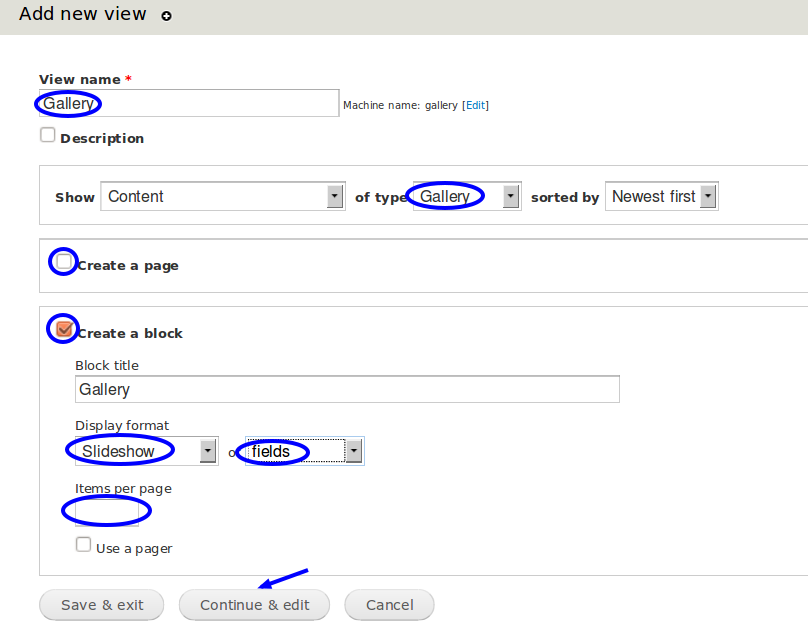
\includegraphics[width=0.650\linewidth]{slideshows-gallery-intro.png}
{\small \begin{enumerate}
\item {} 
View name: Gallery

\item {} 
Show content of type Gallery sorted by Newest first

\item {} 
{[}{]} Uncheck Page

\item {} 
{[}√{]} Check Block

\item {} 
Block title: Gallery

\item {} 
Display fomat: Slideshow of fields

\item {} 
Items per page: (Make this blank)

\item {} 
Continue \& Edit

\end{enumerate}
}\end{figure}
\begin{figure}[htbp]
\centering
\capstart

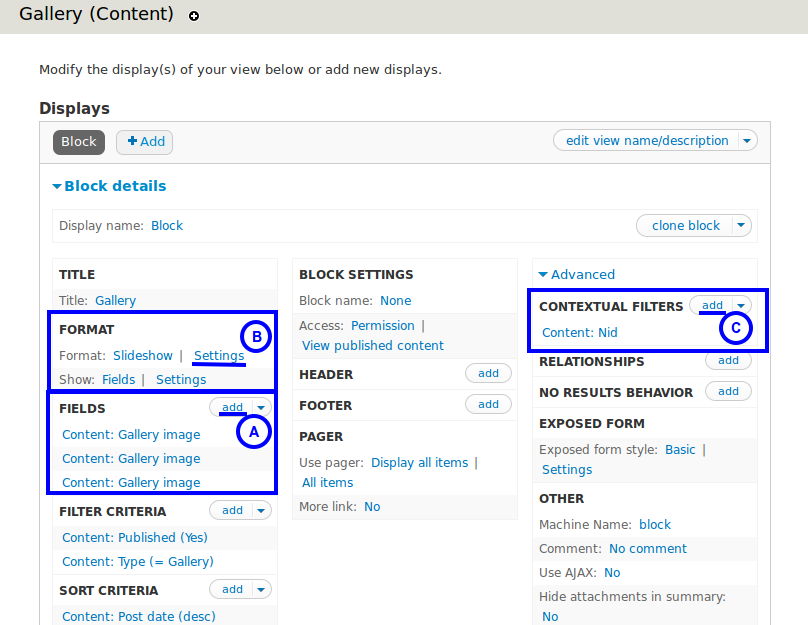
\includegraphics[width=0.650\linewidth]{slideshows-gallery.png}
\caption{In main Views interface, we'll configure three areas:}{\small 
\begin{DUlineblock}{0em}
\item[] A) available fields
\item[] B) row style settings,
\item[] C) the contextual filter.
\end{DUlineblock}

We’ll set them up in this order because they depend upon each other, even though they’re visually in a different order.
}\end{figure}


\subsection{Add Fields}
\label{slideshows:add-fields}
First, add the main gallery image:
\begin{enumerate}
\item {} 
Fields: add

\item {} 
From the popup, select: Content: Gallery image

\item {} 
{[} {]} Remove the check in the box Create a label

\item {} 
Set the Image style to gallery\_main.

\item {} 
Multiple Field Values: {[} {]} Uncheck Display all values in the same row

\item {} 
Apply (All displays)

\end{enumerate}

Second, add the thumbnail gallery images. Much like the first step:
\begin{enumerate}
\item {} 
Fields: add

\item {} 
From the popup, select: Content: Gallery image

\item {} 
{[} {]} Remove the check in the box Create a label

\item {} 
{[}√{]} Check Exclude from display

\item {} 
Set the Image style to gallery\_thumb.

\item {} 
Multiple Field Values: {[} {]} Uncheck Display all values in the same row

\item {} 
Apply (All displays)

\end{enumerate}

Next, add the Alt title.
\begin{enumerate}
\item {} 
Fields: add

\item {} 
From the popup, select:Content: Gallery image

\item {} 
{[} {]} Remove the check in the box Create a label

\item {} 
Leave other visible settings at their default

\item {} 
Multiple Field Values: {[} {]} Uncheck Display all values in the same row

\item {} 
Expand Rewrite Results

\item {} 
{[}√{]} Rewrite the output of this field

\item {} 
In the text field, enter {[}field\_gallery\_image\_2-alt{]} (View the available patterns by expanding Replacement Patterns.)

\item {} 
Apply (all displays)

\end{enumerate}

You now have three fields, all named the same thing but configured differently: the main image, the thumbnails, and the text.

Finally, remove the Content Title since it redundantly displays the name of the gallery.
\begin{enumerate}
\item {} 
Click the link Content: Title

\item {} 
Scroll and click Remove

\end{enumerate}


\subsection{Format}
\label{slideshows:format}\begin{enumerate}
\item {} 
Format: Settings

\item {} 
In the Top Widgets section, check Controls.

\item {} 
In the Bottom Widgets section, check Pager and choose the middle instance of Content: Gallery Image. This will provide the thumbnail images for the pager.

\item {} 
Apply (All displays)

\end{enumerate}


\subsection{Advanced}
\label{slideshows:advanced}\begin{enumerate}
\item {} 
Contextual Filter (Add)

\item {} 
Content: Nid

\item {} 
(∙) Provide a default value \textgreater{} Type: Content ID from URL

\item {} 
Apply (All displays)

\end{enumerate}

Be sure to save the view!


\section{Place and configure the block}
\label{slideshows:place-and-configure-the-block}
\emph{Structure \textgreater{} Blocks \textgreater{} Views: Galleries \textgreater{} Configure}

Configuring the block to display only on Gallery nodes prevents it from being called on a view, and listing it only on specific pages prevents it from appearing on the Edit tab.

Block title:  \textless{}none\textgreater{}

Region Settings
\begin{quote}

Footheme (default theme)
Content
\end{quote}

\textbf{Visibility Settings}

\begin{tabulary}{\linewidth}{|L|L|}
\hline

Pages
 & 
(∙) Only the listed pages (Select this and enter the text below)
galleries*
\\\hline

Content types
 & 
{[}√{]} Gallery (Check only this option)
\\\hline

Roles
 & 
(Leave as is)
\\\hline

Users
 & 
(Leave as is)
\\\hline
\end{tabulary}



\chapter{Create an index of all galleries}
\label{slideshows:create-an-index-of-all-galleries}
\emph{Structure \textgreater{} Views \textgreater{} +Add new view}

You could create the gallery index page in the same view as the gallery block by adding a Page display, but the settings are different enough that they don’t gain a lot by sharing defaults, so we’ll create this as a separate view.


\section{Add a new view}
\label{slideshows:add-a-new-view}

\subsection{Intro screen}
\label{slideshows:intro-screen}\begin{enumerate}
\item {} 
View name: Galleries

\item {} 
Show Content of type Gallery sorted by Newest first

\item {} 
{[}√{]}  Create a page

\item {} 
Page title: Galleries

\item {} 
Display format: Grid of fields

\item {} 
Items to display: 24

\item {} 
{[}√{]}  Create a menu link \textgreater{} Menu: Main menu, Weight: 1

\item {} 
Menu link title: Galleries

\item {} 
Continue \& edit

\end{enumerate}


\subsection{Fields}
\label{slideshows:fields}\begin{enumerate}
\item {} 
add

\item {} 
Gallery image

\item {} 
{[} {]} Uncheck Create a label

\item {} 
Formatter: Image (no change)

\item {} 
Image style: gallery\_index

\item {} 
Link image to: Content

\item {} 
Multiple Field Settings: Accept defaults EXCEPT change Display all value(s) so it reads Display 1 value(s)

\item {} 
Apply (all displays)

\end{enumerate}

Be sure to save the view!


\section{A brief detour}
\label{slideshows:a-brief-detour}
\emph{Structure \textgreater{} Blocks \textgreater{} Main menu: configure}

Footheme uses the block system to place menus, and the main menu is not enabled yet.

Region Settings
\begin{enumerate}
\item {} 
Footheme (default theme). Select Menu Bar.

\item {} 
Save block

\end{enumerate}


\section{Auto-generate galleries}
\label{slideshows:auto-generate-galleries}
\emph{Configuration \textgreater{} Development: Generate content}
\begin{enumerate}
\item {} 
{[}√{]} Gallery (Uncheck others)

\item {} 
Accept the rest of the defaults

\item {} 
Generate

\end{enumerate}

When you're done, visit your gallery index page to see what it looks like when it's populated.


\chapter{Style the Gallery}
\label{slideshows:style-the-gallery}
We'll apply some basic formatting to the galleries.


\section{Open footheme.css}
\label{slideshows:open-footheme-css}
You can edit your style sheet any way that is comfortable for you. If you need more support than the username and password for your sandbox, see Connecting to your sandbox with sFTP at \href{http://training.opensourcery.com/basics/sftp}{http://training.opensourcery.com/basics/sftp}


\section{Arrange thumbnails beneath the main image}
\label{slideshows:arrange-thumbnails-beneath-the-main-image}
\begin{Verbatim}[commandchars=\\\{\}]
/* Arrange the thumbnails beneath the main image */
.views-content-field-gallery-image \PYGZob{}
  float: left;
  padding-right: 13px;
\PYGZcb{}

.views-slideshow-cycle-main-frame-row-item \PYGZob{}
  padding: 5px 20px;
\PYGZcb{}

.views-slideshow-controls-bottom \PYGZob{}
  padding: 0 0 0 20px;
\PYGZcb{}
\end{Verbatim}


\section{Format the controls}
\label{slideshows:format-the-controls}
\begin{Verbatim}[commandchars=\\\{\}]
/* Format the controls */
.views-slideshow-controls-text \PYGZob{}
  padding-left: 20px;
\PYGZcb{}

.views-slideshow-controls-text span \PYGZob{}
  display:  block;
  float: left;
\PYGZcb{}

.views\_slideshow\_controls\_text\_resume,
.views\_slideshow\_controls\_text\_pause\PYGZob{}
  text-align: center;
  width: 55px;
  border-left: 1px solid \#ccc;
  border-right: 1px solid \#ccc;
  padding: 0 5px;
  margin: 0 5px;
\PYGZcb{}
\end{Verbatim}


\section{Place title text over the main image}
\label{slideshows:place-title-text-over-the-main-image}
\emph{Structure \textgreater{} Views \textgreater{} Gallery: edit}

Placing opaque text on a transparent background requires some special setup. If the text is placed inside the transparent container, it will inherit the transparency. Instead, it must be placed parallel to the container and positioned.
\begin{enumerate}
\item {} 
Edit the third instance of the filed content: Galley image

\item {} 
Expand Rewrite Results and edit to match:

\begin{Verbatim}[commandchars=\\\{\}]
\textless{}div class="transparency"\textgreater{}\textless{}/div\textgreater{}
\textless{}div class="overlay"\textgreater{}[field\_gallery\_image\_2-alt]\textless{}/div\textgreater{}
\end{Verbatim}

\item {} 
Apply (all displays)

\item {} 
Add the styling to footheme.css:

\begin{Verbatim}[commandchars=\\\{\}]
/* Overlay the text on the main image */
.views-field-field-gallery-image \PYGZob{}
  position: relative;
\PYGZcb{}

.transparency \PYGZob{}
  position: absolute;
  bottom: -10px;
  left: 0px;
  width: 640px;
  height: 75px;
  background: black;
  margin: 20px;
  filter:alpha(opacity=70);
  opacity: 0.7;
  -moz-opacity:0.7;
\PYGZcb{}

.overlay \PYGZob{}
  color: white;
  position: absolute;
  bottom : 0px;
  left: 0px;
  height: 75px;
  padding: 0 30px 0 30px;
\PYGZcb{}
\end{Verbatim}

\end{enumerate}


\chapter{Set and test permissions}
\label{slideshows:set-and-test-permissions}
\emph{People \textgreater{} Permissions}

If you are not using the Test Kitchen Install Profile or if you are new to the idea of users, roles, permissions or masquerade, see \href{http://training.opensourcery.com/basics}{http://training.opensourcery.com/basics}


\section{Set permissions}
\label{slideshows:set-permissions}
Set permissions as follows:

\begin{tabulary}{\linewidth}{|L|L|L|}
\hline
\textbf{
Author
} & \textbf{
Editor
} & \textbf{
Admin
}\\\hline

{[}√{]} Gallery: Create new content
 & 
{[}√{]} Gallery: Create new content
 & 
{[}√{]} Gallery: Create new content
\\\hline

{[}√{]}  Gallery: Edit own content
 & 
{[} {]}  Gallery: Edit own content
 & 
{[}√{]} Gallery: Edit own content
\\\hline

{[} {]}   Gallery: Edit any content
 & 
{[}√{]} Gallery: Edit any content
 & 
{[}√{]} Gallery: Edit any content
\\\hline

{[}√{]}  Gallery: Delete own content
 & 
{[} {]}  Gallery: Delete own content
 & 
{[}√{]} Gallery: Delete own content
\\\hline

{[} {]}   Gallery: Delete any content
 & 
{[}√{]}  Gallery: Delete any content
 & 
{[}√{]} Gallery: Delete any content
\\\hline
\end{tabulary}



\section{Test Author privileges}
\label{slideshows:test-author-privileges}
Masquerade as Test Author and ensure you CAN:
\begin{enumerate}
\item {} 
Create a gallery

\item {} 
Edit that gallery

\item {} 
Delete that gallery

\end{enumerate}

Ensure you CANNOT:
\begin{enumerate}
\item {} 
Edit galleries you didn’t create

\item {} 
Delete galleries you didn’t create

\end{enumerate}

When you’re done, remember to Switch back


\section{Test Editor privileges}
\label{slideshows:test-editor-privileges}
Masquerade as Test Editor and ensure you CAN:
\begin{enumerate}
\item {} 
Create a gallery

\item {} 
Edit that gallery

\item {} 
Delete that gallery

\item {} 
Edit a gallery you didn’t create

\item {} 
Delete a gallery you didn’t create

\end{enumerate}

raw:: latex
\begin{quote}

begin\{wrapfigure\}\{r\}\{8cm\}  \% ``l'' or ``r'' for the side on the page. And the width parameter for the width of the image space.
centering
includegraphics{[}height=80mm{]}\{\_static/background/note.png\}
caption\{Selbstgebaute „Bluesniper“ um Bluetooth-Geräte aus über 1 km Entfernung anzugreifen. (Stand: 2004)\}
label\{bluesniper\}
end\{wrapfigure\}
\end{quote}


\chapter{Indices and tables}
\label{index:indices-and-tables}\label{index::doc}\begin{itemize}
\item {} 
\emph{genindex}

\item {} 
\emph{modindex}

\item {} 
\emph{search}

\end{itemize}



\renewcommand{\indexname}{Index}
\printindex
\end{document}
